\documentclass[border=4pt]{standalone}
\usepackage{tikz}\usepackage{amssymb}
\usetikzlibrary{positioning,arrows.meta,calc}
\begin{document}
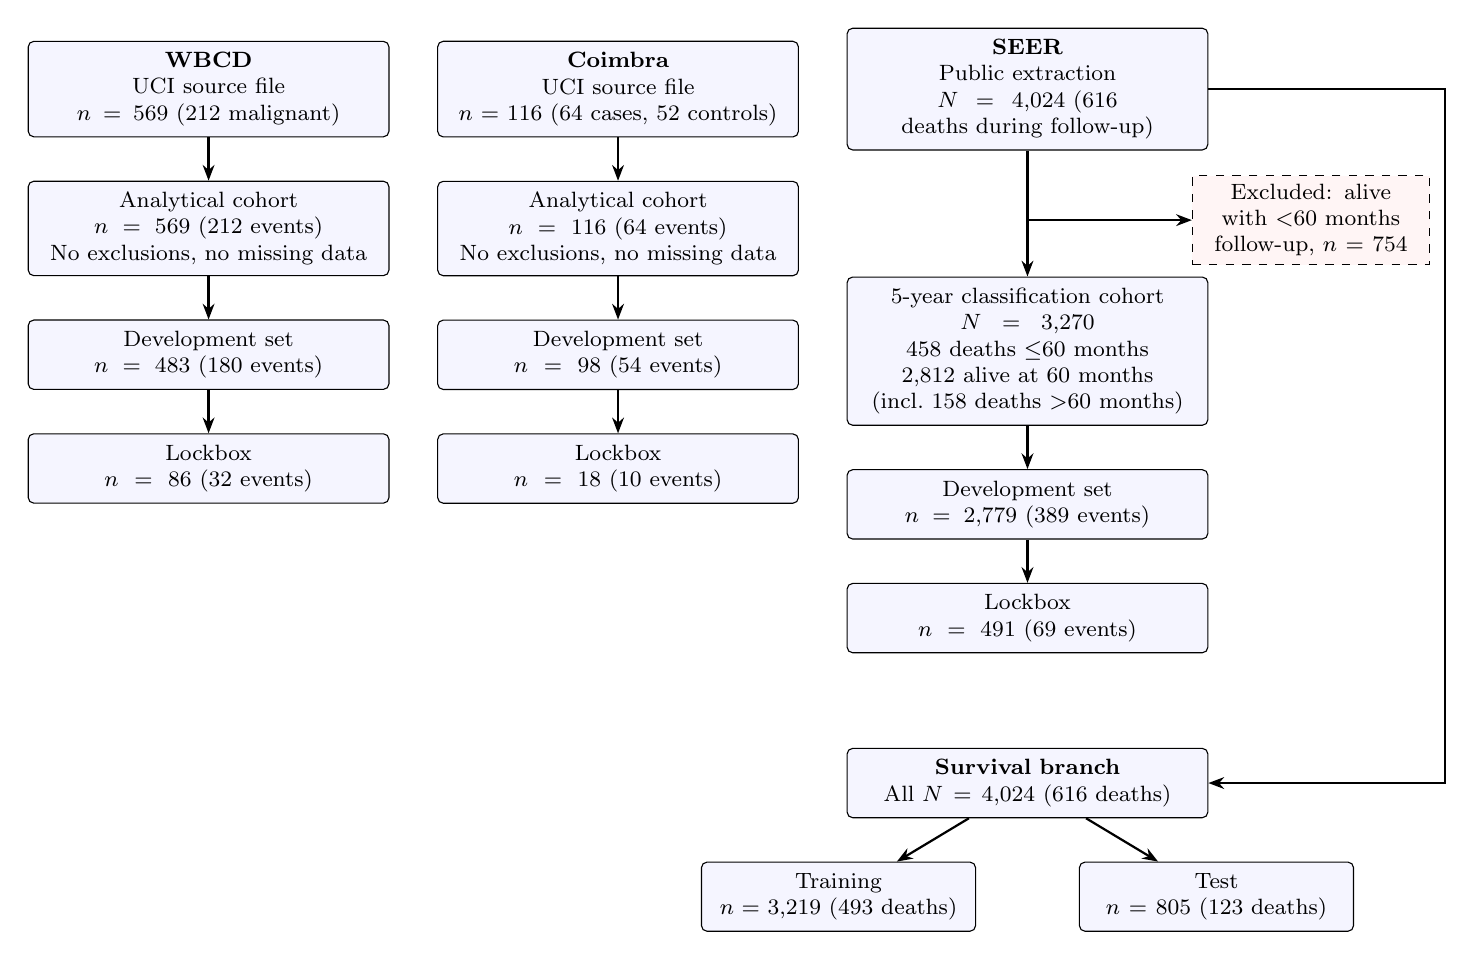
\begin{tikzpicture}[b/.style={draw,rounded corners=2pt,align=center,text width=4.3cm,font=\footnotesize,inner sep=4pt,fill=blue!4},
 e/.style={draw,dashed,align=center,text width=3.4cm,font=\footnotesize,inner sep=3pt,fill=red!4},
 a/.style={-{Stealth[length=2mm]},thick},node distance=0.55cm]
% WBCD
\node[b] (w1) at (0,0) {\textbf{WBCD}\\UCI source file\\$n=569$ (212 malignant)};
\node[b,below=of w1] (w2) {Analytical cohort\\$n=569$ (212 events)\\No exclusions, no missing data};
\node[b,below=of w2] (w3) {Development set\\$n=483$ (180 events)};
\node[b,below=of w3] (w4) {Lockbox\\$n=86$ (32 events)};
\draw[a] (w1)--(w2); \draw[a] (w2)--(w3); \draw[a] (w3)--(w4);
% Coimbra
\node[b] (c1) at (5.2,0) {\textbf{Coimbra}\\UCI source file\\$n=116$ (64 cases, 52 controls)};
\node[b,below=of c1] (c2) {Analytical cohort\\$n=116$ (64 events)\\No exclusions, no missing data};
\node[b,below=of c2] (c3) {Development set\\$n=98$ (54 events)};
\node[b,below=of c3] (c4) {Lockbox\\$n=18$ (10 events)};
\draw[a] (c1)--(c2); \draw[a] (c2)--(c3); \draw[a] (c3)--(c4);
% SEER
\node[b] (s1) at (10.4,0) {\textbf{SEER}\\Public extraction\\$N=4{,}024$ (616 deaths during follow-up)};
\node[b,below=1.6cm of s1] (s2) {5-year classification cohort\\$N=3{,}270$\\458 deaths $\le$60 months\\2,812 alive at 60 months\\(incl.\ 158 deaths $>$60 months)};
\node[e,text width=2.8cm] (ex) at ($(s1)!0.5!(s2)+(3.6,0)$) {Excluded: alive with $<$60 months follow-up, $n=754$};
\draw[a] (s1)--(s2); \draw[a] ($(s1)!0.5!(s2)$)--(ex.west);
\node[b,below=of s2] (s3) {Development set\\$n=2{,}779$ (389 events)};
\node[b,below=of s3] (s4) {Lockbox\\$n=491$ (69 events)};
\draw[a] (s2)--(s3); \draw[a] (s3)--(s4);
\node[b,below=1.2cm of s4] (v1) {\textbf{Survival branch}\\All $N=4{,}024$ (616 deaths)};
\node[b,below=of v1,xshift=-2.4cm,text width=3.2cm] (v2) {Training\\$n=3{,}219$ (493 deaths)};
\node[b,below=of v1,xshift=2.4cm,text width=3.2cm] (v3) {Test\\$n=805$ (123 deaths)};
\draw[a] (s1.east)--++(3.0,0)|-(v1.east);
\draw[a] (v1)--(v2); \draw[a] (v1)--(v3);
\end{tikzpicture}
\end{document}
